Here is an alloy specification of the system described in the RASD:
\lstinputlisting[language=alloy]{Alloy/SeC.als}
\newpage

\begin{figure}[H]
    \begin{center}
        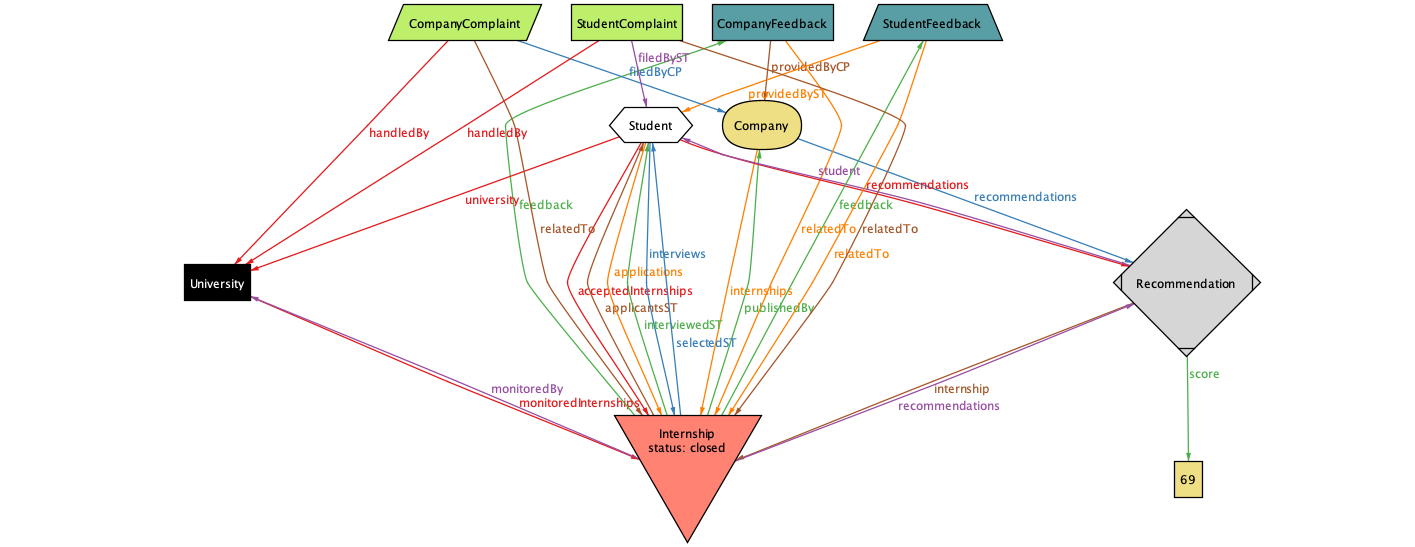
\includegraphics[width=1\linewidth]{Alloy/Base_World.png}
        \caption{Instance for \textit{BaseWorld}.}
        \label{fig:BaseWorld}%
    \end{center}
\end{figure}

\begin{figure}[H]
    \begin{center}
        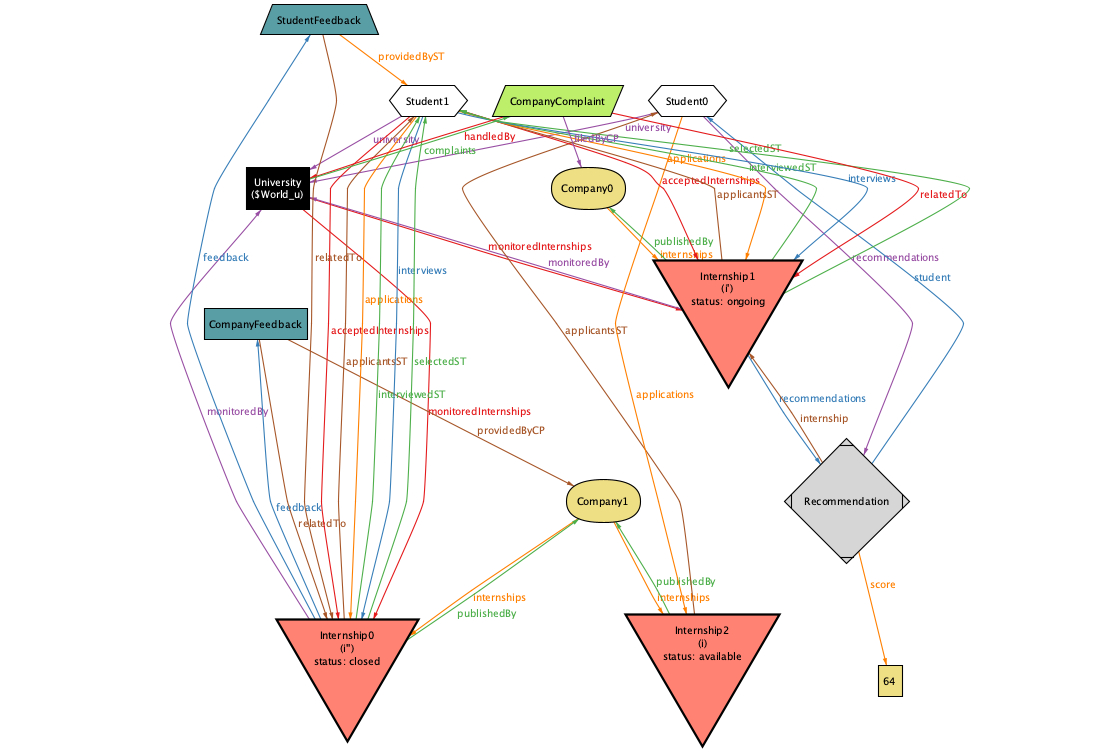
\includegraphics[width=1\linewidth]{Alloy/World_1.png}
        \caption{Instance for \textit{World1}.}
        \label{fig:World1}%
    \end{center}
\end{figure}


\begin{figure}[H]
    \begin{center}
        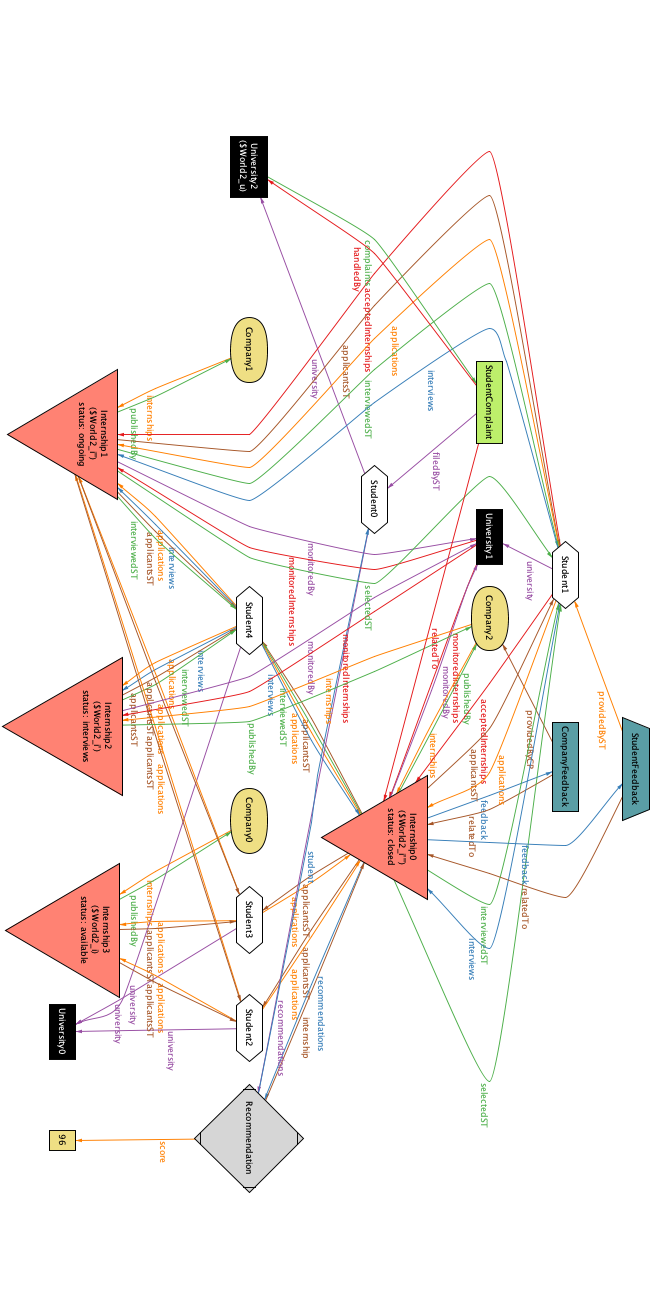
\includegraphics[width=0.7\linewidth]{Alloy/World_2.png}
        \caption{Instance for \textit{World2}.}
        \label{fig:World2}%
    \end{center}
\end{figure}